\chapter{ניהול מצב ודו-כיווניות טקסט}

\section{מנגנוני ניהול מצב בעבודה עם מודלים}

מודלים של שפה גדולים דורשים הנהלה שנתונים זהירה של מצב הקשר שלהם. בעל תפקיד מרכזי כאן הוא תהליך של שמירה על קשר קודם של הקלט כך שהמודל יוכל לשמור על זיכרון של המשיח הקודם. בעזרת מנגנוני תשומת הלב (\textenglish{attention mechanisms}), כל הודעה חדשה בשיחה יכולה להיות זהה כל בדוק עם כל הודעה קודמת, לאפשר מתן תשובות קשורות אל הקשר קודם שלו.

בפרט, מודל \textenglish{Transformer} משתמש בשכבות של תשומת לב לכל זוגות של אסימון אחד כל שני אסימון אחר. זה מאפשר למודל לבנות מפה עמוקה של יחסים בתוך הנתוני קלט.

\begin{equation}
    \text{Attention}(Q, K, V) = \text{softmax}\!\left(\frac{QK^\top}{\sqrt{d_k}}\right)V
\end{equation}

זה הנוסחה לתשומת לב סטנדרטית, שבה \textenglish{Q} היא שאילתה, \textenglish{K} היא מפתח, ו-\textenglish{V} היא ערך. התחזוקה של סטט מהתמונה הקודמת מאפשרת למודל לחזור על הקשר שלו, ובכך לספק תשובות קשורות ויותר טבעיות.

\section{דו-כיווניות בעיבוד טקסט}

עיבוד טקסט בשפות שונות, במיוחד בשפות בעלות כיווניות שונה (כגון עברית, הערבית, והקוריאנית), דורש טיפול מיוחד. תחת טקסט של \textenglish{LTR} (משמאל לימין), כדוגמת \textenglish{English}, הוא מעובד מהשמאל לימין. אך טקסט \textenglish{RTL} (מימין לשמאל), כגון עברית, דורש להיות מעובד בדרך הפוכה.

מערכות המודל של היום, כגון \textenglish{BERT}, \textenglish{GPT}, ו-\textenglish{LLaMA}, בנויות כדי להוציא קוד עם \textenglish{tokenization} המבוססת על תווים או תת-מילים. עבור שפות \textenglish{RTL}, זה יכול ליצור אתגרים בייצוג, ובמיוחד כאשר משדלים טקסט המכיל גם \textenglish{LTR} (כמו שמות אישיים או מונחים טכניים) וגם \textenglish{RTL} (כמו טקסט בעברית).

\begin{LTR}
\begin{verbatim}
def process_bidi_text(text):
    # Detect direction for each segment
    segments = detect_direction_segments(text)
    # Process LTR and RTL separately
    processed = [process_segment(seg, direction) 
                 for seg, direction in segments]
    return combine_segments(processed)
\end{verbatim}
\end{LTR}

עם הבנה זו של דו-כיווניות, אנו יכולים לבנות מערכות שמעבדות טקסט בעברית (ובשפות אחרות של \textenglish{RTL}) בדרך אמינה וביעילות. התהליך דורש הבנה של הן מרכיבי שפה טבעית והן של עקרונות בינאריים בעיצוב מערכות מודרניות.
\begin{figure}[htbp]
    \centering
    % Scaled Dot-Product Attention — canonical anchored LTR-safe version
% \begin{LTR} prevents RTL mirroring from Polyglossia's global RTL context.
% every node/.style includes anchor=center so text sits exactly on each shape.
\begin{LTR}
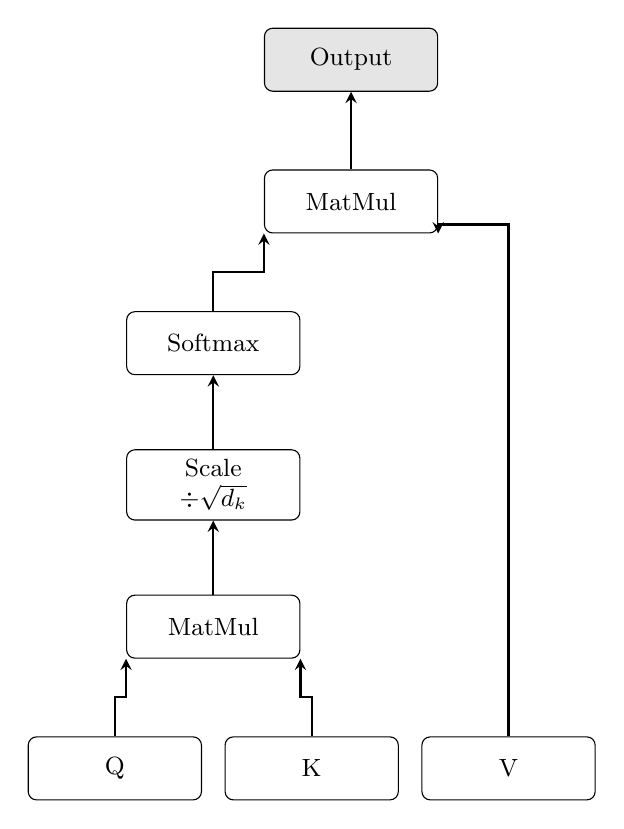
\begin{tikzpicture}[
    every node/.style={
        draw,
        rounded corners=3pt,
        minimum width=2.2cm,
        minimum height=0.8cm,
        align=center,
        anchor=center,
        font=\small
    },
    arrow/.style={->, >=stealth, thick}
]

% Input nodes — bottom row
\node (Q)       at (0,   0) {Q};
\node (K)       at (2.5, 0) {K};
\node (V)       at (5,   0) {V};

% Computation chain (left branch, 1.8 cm vertical spacing > 0.8 cm node height)
\node (matmul1) at (1.25, 1.8) {MatMul};
\node (scale)   at (1.25, 3.6) {Scale \\ \(\div\sqrt{d_k}\)};
\node (softmax) at (1.25, 5.4) {Softmax};

% Merge + output
\node           (matmul2) at (3.0, 7.2) {MatMul};
\node[fill=gray!20] (output)  at (3.0, 9.0) {Output};

% Q and K feed into first MatMul
\draw[arrow] (Q.north) -- ++(0,0.5) -| (matmul1.south west);
\draw[arrow] (K.north) -- ++(0,0.5) -| (matmul1.south east);

% Vertical computation chain
\draw[arrow] (matmul1.north) -- (scale.south);
\draw[arrow] (scale.north)   -- (softmax.south);

% Softmax and V feed into second MatMul
\draw[arrow] (softmax.north) -- ++(0,0.5) -| (matmul2.south west);
\draw[arrow] (V.north)       -- ++(0,6.5) -| (matmul2.south east);

% Final output
\draw[arrow] (matmul2.north) -- (output.south);

\end{tikzpicture}
\end{LTR}

    \caption{ארכיטקטורת \textenglish{Scaled Dot-Product Attention}.}
    \label{fig:sdp_attention}
\end{figure}
